\section{Clustering}


\subsection{Clustering with Gaussian Mixture Model}
One way to cluster data is with a Gaussian Mixture Model (GMM). This model uses a
probabilistic estimation of densities trained, in this report, with the
Expectation Maximizaion (EM) algorithm.\\
The GMM uses multivariate normal distributions as the distribution, which means
each cluster has assigned a mean ($\mu$) and a covariance matrix ($\Sigma$) to it.
This means that a given observation, depending on these two parameters and the
observation itself, has a probability of belonging to each cluster. Then, the
cluster witch the observation is most likely to belong to is the cluster the
observation is assigned to.\\
The first thing to do is find out the amount of clusters the GMM should aim for.
This is done with cross-validation (where the negative log-likehood should be
as low as possibe), Akaike's information Criterion (AIC) and Bayesian Information
Criterion (BIC). AIC and BIC should be low as well, so the following plot, showing
cross-validation, AIC and BIC for different amount of clusters, is helpful when
determining number of clusters.\\
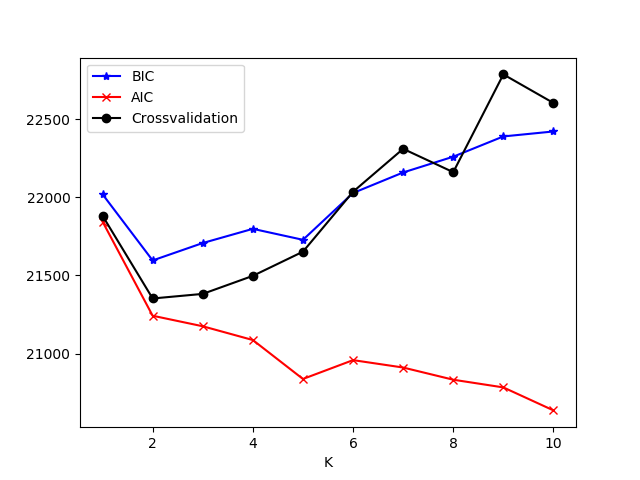
\includegraphics[width=\textwidth]{Figure_1.png}
The BIC and negative log-likelihood are both low at k=2, while AIC continues
decreasing up to k=10. The two criterions penalize model complexity in different ways,
and it is often the case that AIC prefers the more complex model. With this in mind,
k=2 is used for the modelling in this section.\\
The 2 clusters projected down on the 2 attributes explaining the higest amount
of variance (insulin and glucose, responsible for more than 95\% of the total
variance) can be seen below:\\
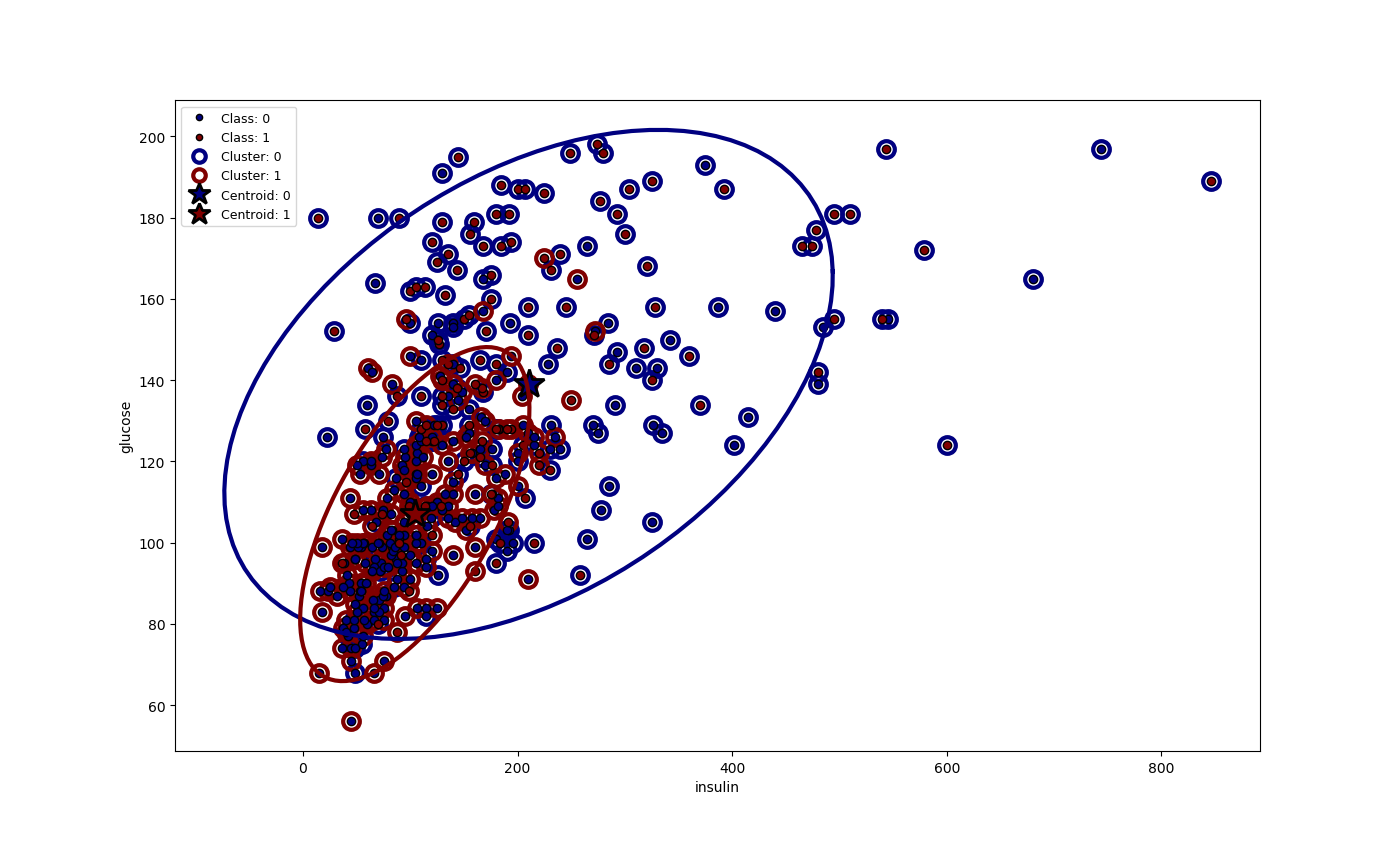
\includegraphics[width=\textwidth]{Figure_2.png}
Qualitatively inspecting the data shows cluster 1 (red circles), which one
will most likely belong when having both low glucose and insulin (centered
at the bottom left red star). Also, cluster 1 seems, in this plane, to be more
an ellipsoid than a circle. Cluster 2 is more spread out and more circular, with
center at higher glucose and insulin levels.

\subsection{Hierarchical clustering}
Hierarchical clustering is a deterministic way of clustering observations. The
point is start off by assigning each observation to its own cluster and then
merge clusters that are closest to each other. Before initializing the algorith,
it is neccessary to




\section{Outlierssssssssss}

\section{Association Miningsssssssss}

\begin{center}
 \begin{tabular}{||c c||}
 \hline
 Attribute number & Attribute \\ [0.5ex]
 \hline\hline
 0 and 9 & Number of times pregnant \\
 \hline
 1 and 10 & Plasma glucose concentration, GTT \\
 \hline
 2 and 11 & Diastolic blood pressure (mm Hg) \\
 \hline
 3 and 12 & Triceps skin fold thickness (mm) \\
 \hline
 4 and 13 & 2-Hour serum insulin ($\mu$ U / ml) \\
 \hline
 5 and 14 & Body mass index Weight in (kg / (Height in $m^2$)) \\
 \hline
 6 and 15 & Diabetes pedigree function \\
 \hline
 7 and 16 & Age (Years) \\
 \hline
 8 and 17 & Class variable, whether or not the person had diabetes (0 or 1) \\ [1ex]
 \hline
\end{tabular}
\end{center}



\appendix
\section{Distribution of responsibilities}
\subsection{Clustering}

\subsection{Outlier detection/Anomaly detection}

\subsection{Association mining}

\subsection{Previous work}
By Hildibjørg.
